\documentclass[12pt,letterpaper]{article}
\usepackage{graphicx}
\usepackage[letterpaper,margin=0.75in]{geometry}

\usepackage{xcolor} % Required for specifying custom colours
\definecolor{grey}{rgb}{0.9,0.9,0.9} % Colour of the box surrounding the title

\usepackage[utf8]{inputenc} % Required for inputting international characters
\usepackage[T1]{fontenc} % Output font encoding for international characters
\usepackage[sfdefault]{ClearSans} % Use the Clear Sans font (sans serif)

\usepackage{tikz}
\usepackage{xstring}
\usepackage{siunitx}



\begin{document}
\newcommand{\getx}[1] {\StrBetween{#1}{(}{,}}
\newcommand{\gety}[1] {\StrBetween{#1}{,}{)}}
%\newcommand{\unpair}[2] {\expandafter\def#2{\getx {#1}}}
\def\mydef#1#2{\def#1{#2}}
\def\uncoord#1#2#3{\def#2{\getx{#1}}\def#3{\gety{#1}}}

\newcommand{\busline}[2] {\draw[thick] #1--#2;}

%----------------------------------------------------------------------------------------
%	TITLE PAGE
%----------------------------------------------------------------------------------------

\begin{titlepage} % Suppresses displaying the page number on the title page and the subsequent page counts as page 1
	
	%------------------------------------------------
	%	Grey title box
	%------------------------------------------------
	
	\colorbox{grey}{
		\parbox[t]{0.93\textwidth}{ % Outer full width box
			\parbox[t]{0.91\textwidth}{ % Inner box for inner right text margin
				\raggedleft % Right align the text
				\fontsize{50pt}{50pt}\selectfont % Title font size, the first argument is the font size and the second is the line spacing, adjust depending on title length
				\vspace{0.7cm} % Space between the start of the title and the top of the grey box
				
				Power Seat \\ 
				Wire Harness\\
				
				\vspace{0.7cm} % Space between the end of the title and the bottom of the grey box
			}
		}
	}

	\parbox[t]{0.93\textwidth}{
		\raggedleft
	    \vspace{0.7cm}
		\textit{Project goals, wire diagram, parts list, dimensions and cost breakdown.}
	}
	\center
    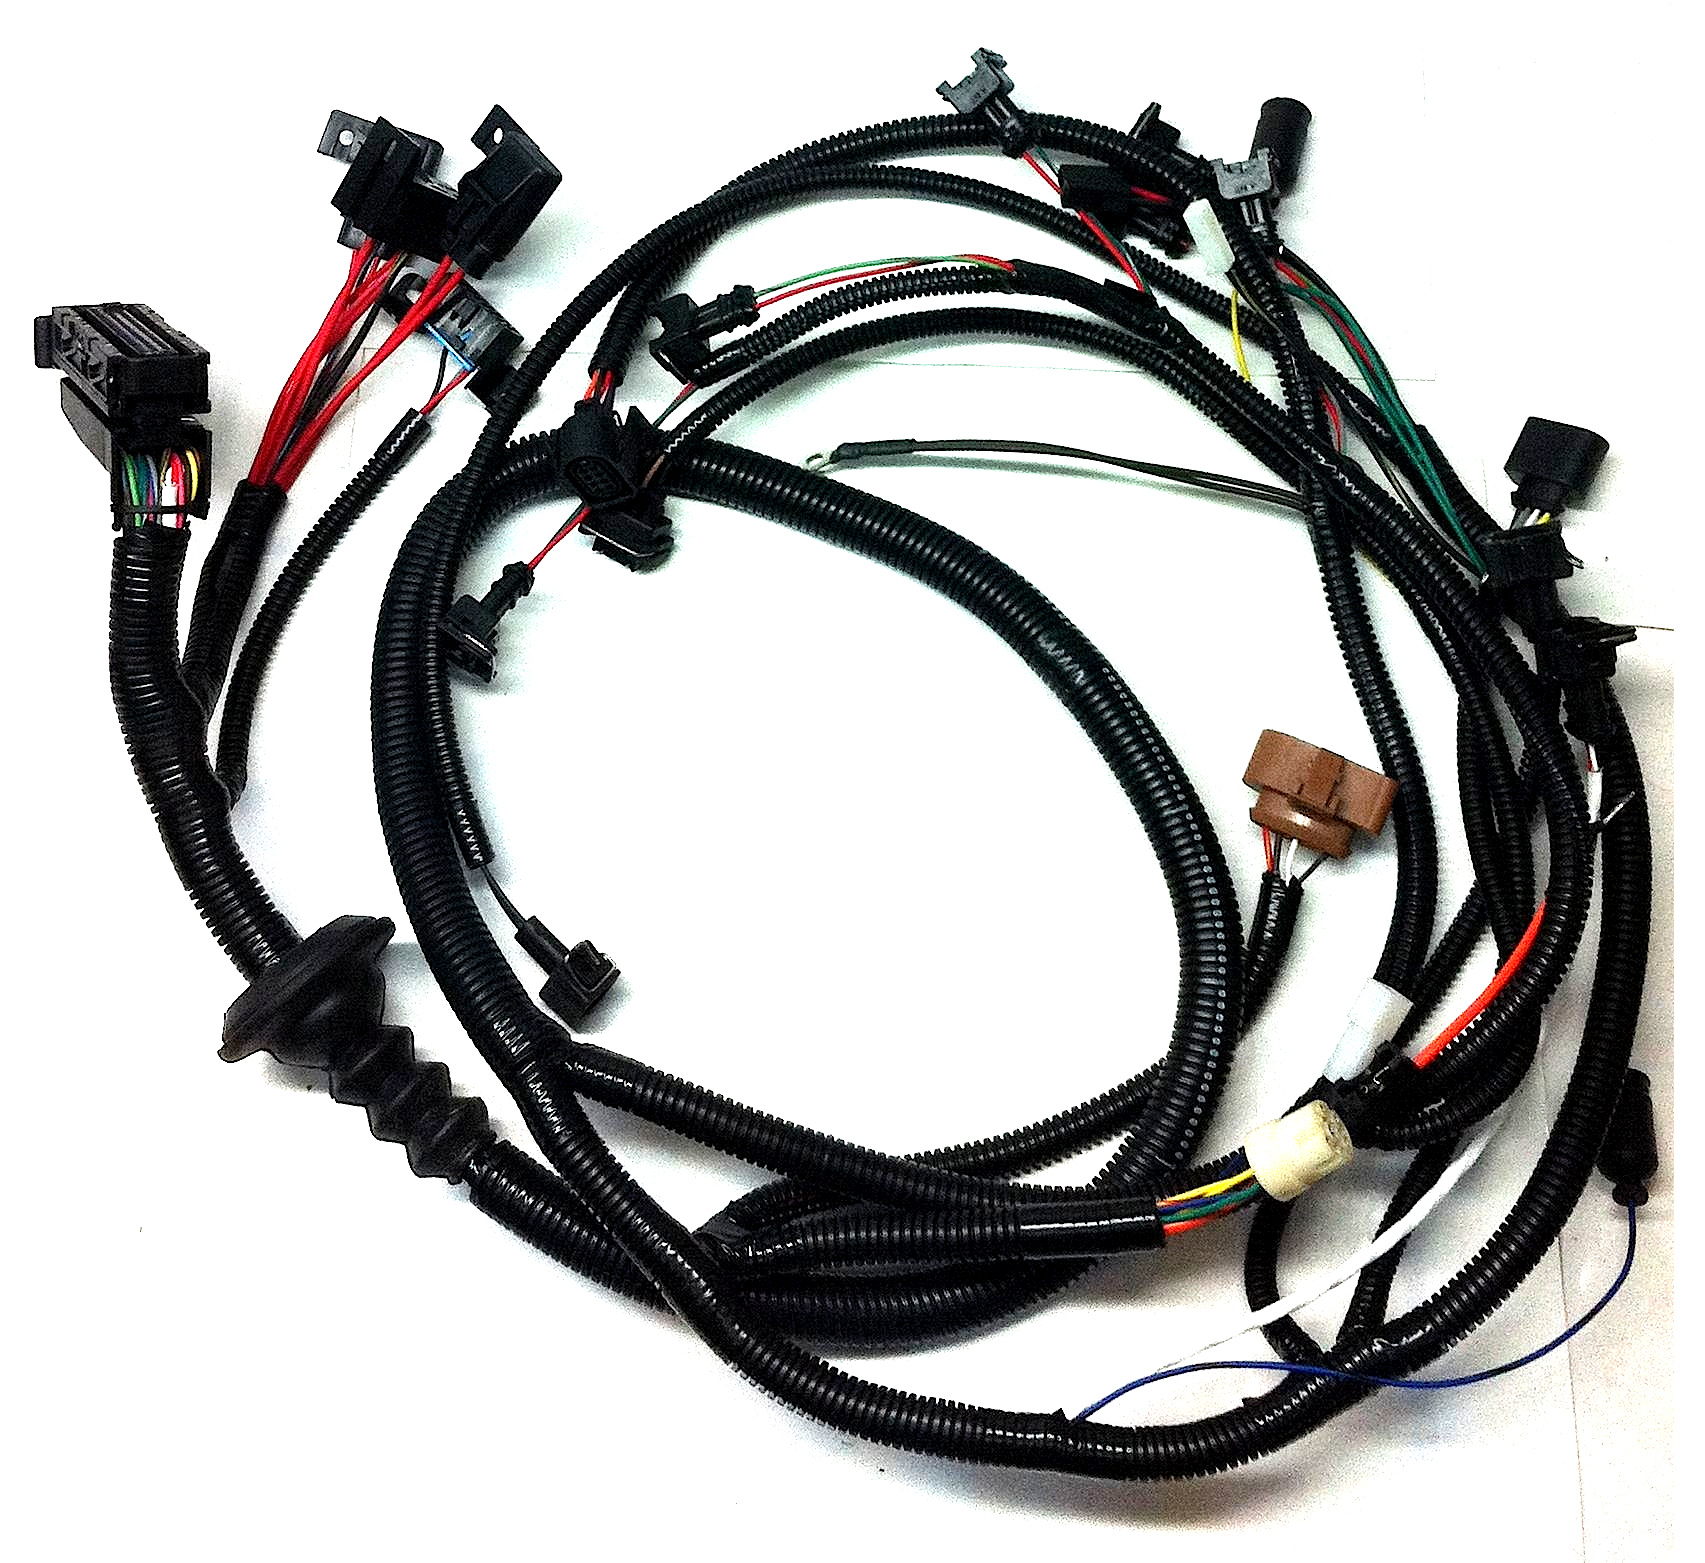
\includegraphics[width=0.70\linewidth]{wireharness.jpg}

	\vfill % Space between the title box and author information
	
	%------------------------------------------------
	%	Author name and information
	%------------------------------------------------
	
	\parbox[t]{0.93\textwidth}{ % Box to inset this section slightly
		\raggedleft % Right align the text
		%\hfill\rule{0.247\linewidth}{1pt}\\% Horizontal line, first argument width, second thickness
		\textit{
		  Vlad Shcherbakov \\
		  November 2017
		}
		
		%\hfill\rule{0.247\linewidth}{1pt}% Horizontal line, first argument width, second thickness
	}
	
\end{titlepage}
\newgeometry{left=0.75in,right=0.75in,top=1in,bottom=0.75in}
\section{Introduction}
The goal of this project is to design a power seat harness for a hypothetical 8-way automotive power seat. Power seats use electrical motors to control seat’s relative positioning within the car, as well as its overall shape. Power controls are often combined with additional manual adjustment mechanisms. The type of a power seat is usually specified by quantifying the number of ways it can be adjusted using power controls. This number does not include the number of ways a seat can be adjusted using manual controls and does not alone specify which controls are manual and which are powered. Thus not all 8-way power seats are alike.

Our hypothetical power seat, will have power adjustable \textit{bottom height}, \textit{bottom angle}, \textit{seat distance} from the steering wheel and \textit{lumbar support}. That’s total of 4 adjustable parameters. Since each one of the 4 parameters can be adjusted in 2 ways(increased or decreased) there are total of 8 ways in which seat can be adjusted. In addition to 4 power adjustments, there’s going to be one more manual adjustment: \textit{seatback recline}.
\begin{figure}[b!]
  \centering
  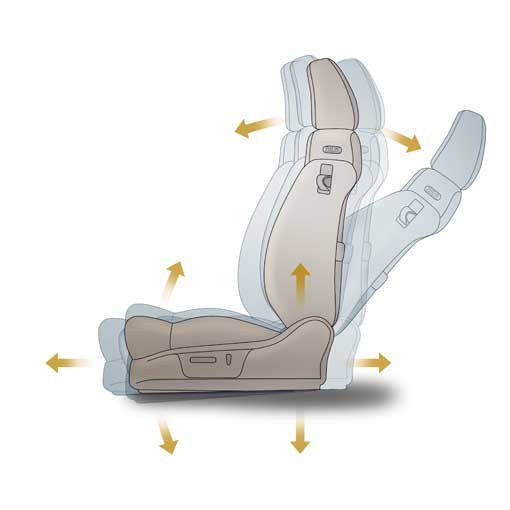
\includegraphics[width=0.70\linewidth]{8-way-seat.jpg}
  \caption{8-way power seat with manual backseat recline adjustment.}
  \label{fig:wireharness1}
\end{figure}
\newpage
\newgeometry{margin=0.75in}
\section{Electrical Interface}
The role of the power seat wire harness is to conduct electrical current between \textit{power source}, mechanical \textit{switch assemblies} and electrical \textit{motors}. Our power seat uses \textit{4 electrical motors} and \textit{2 switch assemblies}. The switch assemblies control which electrical motors receive electrical current as well as in which direction it is flowing for each motor.

The first switch assembly is used just for \textit{lumbar support} and controls only one motor, while the second switch assembly controls the other 3 motors, for \textit{height}, \textit{angle} and \textit{distance} adjustments.

The motors used are all \textit{Direct Current} and each is a two-terminal device. Each motor is usually dedicated to adjusting a single parameter, with the exception of \textit{angle} and \textit{height}. Neither of those two parameters are controlled by any single motor, but by two motors working simultaneously: one raises(or lowers) the front and the other the back of the seat.

The power is supplied from without by a lead-acid battery over two terminals, usually with 12\si{\volt} potential between them and hopefully with a fuse somewhere in series as the only current limiting device. 

Each switch assembly requires two power inputs, for both ground and positive potential, meaning a total of 4 power lines is needed. This is a problem, because the power terminal of the car supplies only 2. Additional 2 power lines will have to be spliced from the 2 existing ones in order to supply power for the second switch assembly.

\newpage

\section{Geometrical Constraints}



Angle and height adjustments are performed by by raising(or lowering) the front and the back of a seat. One motor is used for the front and another for the back.




The requirement to control direction of the current makes it impossible to connect all motors to common ground and will double the number of wires running between switch assemblies and electrical motors.

TODO:\\
Explain configuration of the motors and how they achieve performing the 4 power adjustments.
Explain how a switch assembly might be simulated on a circuit level, to improve understanding.\\
Provide drawing showing how the final harness will look when installed, showing positions of motors and switch assemblies and the seat.\\
Provide parts list. Parts list should also provide dimensions for wire and loome cuts, and the wire diagram will explain how they must be connected.
Summarize total cost in parts and assembly time per unit.


\nopagebreak 
\begin{figure}[h]
\centering
\def\svgwidth{0.5\columnwidth}
\input{776532-3.pdf_tex}
\end{figure}
\clearpage

% \def\scl{0.6}%scaling factor of the picture
% \begin{tikzpicture}[
%   scale=\scl,
%   controlpanels/.style={yellow!30!brown!20!,rounded corners,draw=black,thick},
%   screen/.style={green!50!black!60!,draw=black,thick},
%   trace/.style={green!60!yellow!40!, ultra thick},
%   smallbutton/.style={white,draw=black, thick},
%   axes/.style={thick}]
%   \fill[green!30!blue!30!,rounded corners,draw=black,thick](0,0)
%     rectangle (27.75,13.25);
%   \fill[fill=black!40!,draw=black,thick,rounded corners](0.25,0.25)
%     rectangle (27.5,13.00);
%   % Screen, centered around the origin then shifted for easy plotting
%   \begin{scope}[xshift=7cm,yshift=8cm,samples=150]
%     \fill[black!60!,rounded corners,draw=black,thick](-5.3,-4.3)
%       rectangle (5.3,4.3);
%     \fill[screen] (-5.0,-4.0) rectangle (5.0,4.0);
%     \draw[trace] plot(\x,{1+2.4*sin((2.5*\x +1) r)}); % r for radians...
%     \draw[trace] plot(\x,{-1+1.25*sin((0.75*\x) r});
%     \draw[thin] (-5.0,-4.0) grid (5.0,4.0);
%     \draw[axes] (-5,0)--(5,0); % Time axis
%     \draw[axes] (0,-4)--(0,4);
%     \foreach \i in {-4.8,-4.6,...,4.8} \draw (\i,-0.1)--(\i,0.1);
%     \foreach \i in {-3.8,-3.6,...,3.8} \draw (-0.1,\i)--(0.1,\i);
%   \end{scope}
%   % Feet
%   \fill[black!70!,rounded corners,xshift=2cm] (0,-.5) rectangle (2,0);
%   \fill[black!70!,rounded corners,xshift=23.75cm] (0,-.5) rectangle (2,0);
%   % Lower left panel
%   \fill[controlpanels] (0.6,0.5) rectangle (13.5,3.0);
%   \path (0.8,0.9) node[scale=\scl,right]{$\mathbf{TeXtronics\,1 - v.1.01}$};
%   % Lower right panel
%   \fill[controlpanels] (13.7,0.5) rectangle (27.1,6.2);
%   %Channels
%   % CH I
%   \draw[thick] (14.8,1.5) circle (0.7cm);
%   \fill[gray,draw=black,thick] (14.8,1.5) circle (0.5cm);
%   \fill[white,draw=black,thick] (14.8,1.5) circle (0.3cm);
%   \node[scale={1.5*\scl}] at (14.8,2.5) {CH I};
%   \draw[thick] (16.2,1.5) circle (0.4cm);
%   \fill[black!60!] (16.2,1.5) circle (0.3cm);
%   \draw[thick] (16.6,1.5) --(17,1.5)--(17,1.0);
%   \draw[thick] (16.7,1.0)--(17.3,1.0);
%   \draw[thick] (16.8,0.85)--(17.2,0.85);
%   \draw[thick] (16.9,0.70)--(17.1,0.70);
%   \draw[thick] (26.0,1.5) circle (0.7cm);
%   % CH II
%   \fill[gray,draw=black,thick] (26,1.5) circle (0.5cm);
%   \fill[white,draw=black,thick] (26,1.5) circle (0.3cm);
%   \node[scale={1.5*\scl}] at (26,2.5) {CH II};
%   \draw[thick] (24.6,1.5) circle (0.4cm);
%   \fill[black!60!] (24.6,1.5) circle (0.3cm);
%   \draw[thick] (24.2,1.5) --(23.7,1.5)--(23.7,1.0);
%   \draw[thick] (23.4,1.0)--(24.0,1.0);
%   \draw[thick] (23.5,0.85)--(23.9,0.85);
%   \draw[thick] (23.6,0.70)--(23.8,0.70);
%   \draw[thick] (26.0,1.5) circle (0.7cm);
%   % Y-pos
%   \fill[smallbutton] (14.8,4.9) circle (0.3cm);
%   \node[scale={\scl}] at (14.8,5.5) {Y-pos I};
%   \fill[smallbutton] (26.0,4.9) circle (0.3cm);
%   \node[scale={\scl}] at (26.0,5.5) {Y-pos II};
%   % Volt/div the foreach loop draws the two buttons
%   \foreach \i / \b in {18/75,22.5/345}{
%   %Second parameter of the loop is the angle of the index mark 
%   \begin{scope}[xshift=\i cm,yshift=3.8cm,scale=0.85]
%     \node[scale=\scl] at (0,2.3) {Volts/Div};
%     \node[scale=\scl,black] at (-1,-2.4) {V};
%     \node[scale=\scl,blue]  at (1,-2.4) {mV};
%     \clip[rounded corners] (-2,-2) rectangle (2,2);
%     \fill[black!30!,rounded corners,draw=black,thick] (-2,-2)
%       rectangle (2,2);
%     \fill[blue!50!black!20!,draw=black,thick]
%       (30:1.1)--(30:3)--(3,-3)--(-90:3)--(-90:1.1) arc (-90:30:1.1);
%     \draw[very thick,rounded corners](-2,-2) rectangle (2,2);
%     \draw[thick] (0,0) circle (1.0);
%     \foreach \i in {0,30,...,330}
%       \draw[thick] (\i:1.2)--(\i:2.5);
%     \foreach \i/\j in {15/50,45/.1,75/.2,105/.5,135/1,165/2,195/5,225/10,
%       255/20,285/5,315/10,345/20} \node[scale=\scl,black] at (\i:1.7) {\j};
%     \fill[blue!30!black!60!,draw=black,thick] (0,0) circle (0.8cm);
%     % Here you set the right Volts/Div button
%     \draw[ultra thick,red] (\b:0.3)--(\b:1.2);
%   \end{scope}}
% % Upper right panel
%   \fill[controlpanels] (13.7,6.5) rectangle (27.1,12.75);
%   %On-Off button
%   \draw[rounded corners,thick,blue] (13.9,10.5) rectangle (15.9,12.5);
%   \fill[fill=red,draw=black,thick,rounded corners] (14.4,10.8) rectangle (15.3,11.2);
%   \node[scale=\scl] at (14.8,12) {\textbf{Power}};
%   \node[scale=\scl] at (14.8,11.5) {\textbf{On/Off}};
%   % Focus-Intensity buttons
%   \draw[rounded corners,thick,blue] (13.9,7.0) rectangle (15.9,10.0);
%   \fill[smallbutton] (14.9,7.5) circle (0.3cm);
%   \node[scale=\scl] at (14.9,8.2) {\textbf{Focus}};
%   \fill[smallbutton] (14.9,9) circle (0.3cm);
%   \node[scale=\scl] at (14.9,9.6) {\textbf{Intens}};
%   % X-pos
%   \fill[smallbutton] (24.5,9.9) circle (0.3cm);
%   \node[scale={\scl}] at (24.5,10.5) {X-pos};
%   % Time/Div
%   \begin{scope}[xshift=21cm,yshift=9.5cm,scale=1]
%     \node[scale={1.25*\scl}]  at (0,2.4) {Time/Div};
%     \clip[rounded corners] (-2.2,-2) rectangle (2.2,2);
%     \fill[black!30!,rounded corners,draw=black,thick] (-2.2,-2) rectangle (2.2,2);
%     \fill[blue!50!black!20!,draw=black,thick]
%       (45:1.1)--(45:3)--(3,-3)--(-90:3)--(-90:1.1) arc (-90:45:1.1);
%     \fill[green!50!black!40!,draw=black,thick]
%       (45:1.1)--(45:3) arc(45:207:3) --(207:1.1) arc (207:45:1.1);
%     \draw[very thick,rounded corners](-2.2,-2) rectangle (2.2,2);
%     \node[scale={1.25*\scl}] at (-1.6,-1.6) {$s$};
%     \node[scale={1.25*\scl}] at (1.6,-1.6) {$\mu{}\,s$};
%     \node[scale={1.25*\scl}] at (-1.6,1.6) {$m\,s$};
%     \draw[thick] (0,0) circle (1.0);
%     \foreach \i in {-72,-54,...,262} \draw[thick] (\i:1.15)--(\i:1.35);
%     \foreach \i/\j in {-72/.5,-54/1,-36/2,-18/5,0/10,18/20,36/50,54/.1,72/.2,90/.5,
%       108/1,126/2,144/5,162/10,180/20,198/50,216/.1,234/.2,252/.5}
%       \node[scale=\scl,black] at (\i:1.7){\j};
%     \fill[blue!30!black!60!,draw=black,thick] (0,0) circle (0.8cm);
%     % Here you set the Time/Div button
%     \draw[ultra thick,red] (-18:0.3)--(-18:1.2);	
%     % X-pos
%   \end{scope}
% \end{tikzpicture}
\end{document}
